%%%%%%%%%%%%%%%%%%%%%%%%%%%%%%%%%%%%%%%%%
% Research project proposal template
% Based on:
%
% LaTeX Template
% Version 2.5 (27/8/17)
%
% This template was downloaded from:
% http://www.LaTeXTemplates.com
%
% Version 2.x major modifications by: 
% Helen Robertson
%
% With thanks to:
% Matthew Woolway and Terence Van Zyl for help with coding and content.
%
% This template is based on a template by:
% Steve Gunn (http://users.ecs.soton.ac.uk/srg/softwaretools/document/templates/)
% Sunil Patel (http://www.sunilpatel.co.uk/thesis-template/)
%
% Template license:
% CC BY-NC-SA 3.0 (http://creativecommons.org/licenses/by-nc-sa/3.0/)
% 
% This template has been constructed in accordance with the requirements and conventions of the School of Computer Science and Applied Mathematics and of the Faculty of Science at the University of the Witwatersrand.
%
%%%%%%%%%%%%%%%%%%%%%%%%%%%%%%%%%%%%%%%%%

%----------------------------------------------------------------------------------------
%	PACKAGES AND OTHER DOCUMENT CONFIGURATIONS
%----------------------------------------------------------------------------------------

\documentclass[
12pt, % The default document font size, options: 10pt, 11pt, 12pt
oneside, % Two side (alternating margins) for binding by default, uncomment to switch to one side
english, % ngerman for German
onehalfspacing, % One-and-a-half line spacing, alternatives: singlespacing or doublespacing
%draft, % Uncomment to enable draft mode (no pictures, no links, overfull hboxes indicated)
nolistspacing, % If the document is onehalfspacing or doublespacing, uncomment this to set spacing in lists to single
liststotoc, % Uncomment to add the list of figures/tables/etc to the table of contents
%toctotoc, % Uncomment to add the main table of contents to the table of contents
%parskip, % Uncomment to add space between paragraphs
%nohyperref, % Uncomment to not load the hyperref package
headsepline, % Uncomment to get a line under the header
%chapterinoneline, % Uncomment to place the chapter title next to the number on one line
%consistentlayout, % Uncomment to change the layout of the declaration, abstract and acknowledgements pages to match the default layout
]{ProposalAndThesis} % The class file specifying the document structure
\usepackage{tabularx}

\usepackage[utf8]{inputenc} % Required for inputting international characters
\usepackage[T1]{fontenc} % Output font encoding for international characters
\usepackage{mathpazo} % Use the Palatino font by default
\usepackage{amsmath}
\usepackage[backend=biber,style=numeric,natbib=true]{biblatex} % Use the bibtex backend with the numeric citation style
\hfuzz=2pt % Ignores all overfull hbox warnings less than 2pt long
\usepackage{pdflscape}
\usepackage{multirow}
\addbibresource{main.bib} % The filename of the bibliography

\usepackage[autostyle=true]{csquotes} % Required to generate language-dependent quotes in the bibliography

\usepackage[cleanlook, english]{isodate} % Required for UK date formatting
\usepackage{fancybox} % Required for boxed text sections
\usepackage{xcolor} % Required for coloured text

\usepackage{pgfgantt}

\definecolor{ShadowColor}{RGB}{0,103,165} % Required for coloured shadow in boxed text sections
\makeatletter
\newcommand\Cshadowbox{\VerbBox\@Cshadowbox}
\def\@Cshadowbox#1{%
	\setbox\@fancybox\hbox{\fbox{#1}}%
	\leavevmode\vbox{%
		\offinterlineskip
		\dimen@=\shadowsize
		\advance\dimen@ .5\fboxrule
		\hbox{\copy\@fancybox\kern.5\fboxrule\lower\shadowsize\hbox{%
				\color{ShadowColor}\vrule \@height\ht\@fancybox \@depth\dp\@fancybox \@width\dimen@}}%
		\vskip\dimexpr-\dimen@+0.5\fboxrule\relax
		\moveright\shadowsize\vbox{%
			\color{ShadowColor}\hrule \@width\wd\@fancybox \@height\dimen@}}}
\makeatother

%----------------------------------------------------------------------------------------
%	MARGIN SETTINGS
%----------------------------------------------------------------------------------------

\geometry{
	paper=a4paper, % Change to letterpaper for US letter
	inner=2.8cm, % Inner margin
	outer=2.8cm, % Outer margin
	bindingoffset=0.0cm, % Binding offset
	top=2.8cm, % Top margin
	bottom=2.8cm, % Bottom margin
	%showframe, % Uncomment to show how the type block is set on the page
}

%----------------------------------------------------------------------------------------
%	THESIS INFORMATION
%----------------------------------------------------------------------------------------

\thesistitle{A Simulation-based comparison of the predictive accuracy of the random survival forest and the lasso-regularized Cox Model in Survival Analysis} % Your thesis title, this is used in the title and abstract, print it elsewhere with \ttitle
\supervisor{Dr. Alphonce Bere} % Your supervisor's name, this is used in the title page, print it elsewhere with \supname
% \cosupervisor{Name of Co-supervisor Here (or Delete)} % Your co-supervisor's name, this is used in the title page, print it elsewhere with \cosupname
%\examiner{} % Your examiner's name, this is not currently used anywhere in the template, print it elsewhere with \examname
\degree{Master of Science, Artificial Intelligence} % Your degree name, this is used in the title page and abstract, print it elsewhere with \degreename
\author{Willem Van Der Merwe} % Your name, this is used in the title page and abstract, print it elsewhere with \authorname
%\addresses{} % Your address, this is not currently used anywhere in the template, print it elsewhere with \addressname
%\subject{} % Your subject area, this is not currently used anywhere in the template, print it elsewhere with \subjectname
%\keywords{} % Keywords for your thesis, this is not currently used anywhere in the template, print it elsewhere with \keywordnames
\university{University of the Witwatersrand, Johannesburg} % Your university's name, this is used in the title page and abstract, print it elsewhere with \univname
\department{Faculty of Science} % Your department's name, this is used in the title page and abstract, print it elsewhere with \deptname
%\group{\href{http://research group.com}{Research Group Name}} % Your research group's name and URL, this is not currently used anywhere in the template, print it elsewhere with \groupname
%\faculty{\href{http://faculty.university.com}{Faculty Name}} % Your faculty's name and URL, this is not currently used anywhere in the template, print it elsewhere with \facname

\def\keywordnames{Appendices; Chapters; Figures; example.bib; main.pdf; main.tex; main.bbl; main.aux; main.blg; main.lof; main.log; main.lot; main.out; MastersDoctoralThesis.cls}

\newcommand{\keyword}[1]{\textbf{#1}}
\newcommand{\tabhead}[1]{\textbf{#1}}
\newcommand{\code}[1]{\texttt{#1}}
\newcommand{\file}[1]{\texttt{\bfseries#1}}
\newcommand{\option}[1]{\texttt{\itshape#1}}



\AtBeginDocument{
\hypersetup{pdftitle=\ttitle} % Set the PDF's title to your title
\hypersetup{pdfauthor=\authorname} % Set the PDF's author to your name
\hypersetup{pdfkeywords=\keywordnames} % Set the PDF's keywords to your keywords
}

\begin{document}

\frontmatter % Use roman page numbering style (i, ii, iii, iv...) for the pre-content pages

\pagestyle{plain} % Default to the plain heading style until the thesis style is called for the body content

%----------------------------------------------------------------------------------------
%	TITLE PAGE
%----------------------------------------------------------------------------------------

\begin{titlepage}
\begin{center}

{\large \bfseries \ttitle}\par\vspace{0.4cm} % Thesis title
\HRule\par\vspace{1.5cm}
\authorname\par\vspace{1cm}
\emph{Supervisor(s):}\par
{\supname}\par % Name of supervisor
% {\cosupname} % Name of co-supervisor
\par\vspace{0.5cm}


\includegraphics[width=80mm]{Figures/logoWitsstackedcolourtransparent.png} % University crest
\vfill

A research proposal submitted in partial fulfillment of the requirements for the degree of \degreename\par\vspace{0.3cm}
in the\par\vspace{0.4cm}
\deptname\par\vspace{0.1cm} % Name of department
\univname\par\vspace{0.4cm} % Name of university
\cleanlookdateon
\today % Date

\end{center}

\end{titlepage}

%---------------------------------------------------------------------------------------
%	USING THIS TEMPLATE
%---------------------------------------------------------------------------------------

% \par\vspace{0.5cm}
% \noindent \Cshadowbox{
% 	\begin{minipage}{15cm}
% 		\medskip
% 		\color[rgb]{0.0,0.4,0.65} 
% 		\begin{center} 
% 			\medskip \textbf{Using this template} \par 
% 			\end{center}
% 			\medskip The template below has been constructed in line with the Faculty of Science requirements as well as the conventions of the School. Guidance on each section can be found in the blue boxes at the start of the section. Note that conventions and preferences for structuring a research proposal can vary from discipline to discipline and supervisor to supervisor. Both the template and the guidance on the different sections are suggestions for structuring the proposal. If your supervisor has a different preferred convention or template, it is recommended that you consult with them regarding the differences. \par \medskip
% 			Further details on using the template can be found in Appendix B. \par \medskip
% 			You should ensure that you either delete or comment out the blue boxes before submission of the proposal. \par
% 		\medskip 
% \end{minipage}}\\ 

%----------------------------------------------------------------------------------------
%	DECLARATION PAGE
%----------------------------------------------------------------------------------------

\begin{declaration}
\addchaptertocentry{\authorshipname} % Add the declaration to the table of contents
\vspace{0.5cm}
\noindent I, \authorname, declare that this proposal is my own, unaided work. It is being submitted for the degree of {\degreename} at the \univname. It has not been submitted for any degree or examination at any other university.

\par\vspace{2cm}
\begin{flushright}

\includegraphics[width=30mm]{Figures/sign.png}\par 
\authorname\par\vspace{0.1cm}
\today
\end{flushright}

% \par\vspace{0.5cm}
% \noindent \Cshadowbox{
% 	\begin{minipage}{15cm}
% 		\medskip
% 		\color[rgb]{0.0,0.4,0.65} 
% 		\medskip The declaration is an important formal requirement. Ensure that you upload an
% 		image of your signature and that you change the file name in the main.tex file to include it.
% 		\medskip 
% \end{minipage}}\\ 

\end{declaration}
\vfill
\pagebreak

%----------------------------------------------------------------------------------------
%	QUOTATION PAGE
%----------------------------------------------------------------------------------------

%\vspace*{0.2\textheight}

%\noindent\enquote{\itshape Thanks to my solid academic training, today I can write hundreds of words on virtually any topic without possessing a shred of information, which is how I got a good job in journalism.}\bigbreak

%\hfill Dave Barry

%----------------------------------------------------------------------------------------
%	ABSTRACT PAGE
%----------------------------------------------------------------------------------------

\begin{abstract}
\addchaptertocentry{\abstractname} % Add the abstract to the table of contents
\begin{quote}
This proposal aims to study critical gaps in comparative simulation studies within survival analysis, highlighting the need for rigorous methodological frameworks and improved replicatable standards. Despite the widespread application of survival models within traditional and machine learning contexts for predicting event times, discrepancies in method implementation and evaluation can lead to biased outcomes and limit the generalizability of findings. This study aims to conduct a comprehensive comparative analysis of established survival models, specifically Random Survival Forest and Lasso-Cox models, using both simulated and real datasets. By adhering to the ADMEP framework and employing advanced data-generating mechanisms, this research seeks to provide empirical insights into the models' behavior and effectiveness under varied conditions. I aim to enhance the reliability of survival predictions and contribute to methodological standards in survival analysis, addressing the prevalent issues of inadequate design, reporting, and the need for methodological rigor in simulation studies.
\end{quote}

% \par\vspace{0.5cm}
% \noindent \Cshadowbox{
%     \begin{minipage}{15cm}
%     \bigskip
%     \color[rgb]{0.0,0.4,0.65}The abstract is a brief informative summary of the proposed research. It can be read independently and should 
%     	\begin{itemize}
%     		\item locate the proposed research within the background relevant to it,
%     		\item state the research question or aim,
%     		\item briefly describe the proposed methods for answering the question or achieving the aim, and,
%     		\item emphasise the contribution that the proposed research will make to current research in the field.
%     	\end{itemize}
%     	It is recommended that your abstract is no more than 300 words.
%     \medskip
% 	\end{minipage}}

\end{abstract}

%----------------------------------------------------------------------------------------
%	ACKNOWLEDGEMENTS
%----------------------------------------------------------------------------------------

% \begin{acknowledgements}
% \addchaptertocentry{\acknowledgementname} % Add the acknowledgements to the table of contents
% \vspace{0.5cm}
% \noindent{Lorem ipsum dolor sit amet, consectetur adipiscing elit. Aliquam ultricies lacinia euismod. Nam tempus risus in dolor rhoncus in interdum enim tincidunt. Donec vel nunc neque.}

% \par\vspace{0.5cm}
% \noindent \Cshadowbox{
% 	\begin{minipage}{15cm}
% 		\medskip
% 		\color[rgb]{0.0,0.4,0.65} 
% 		\medskip The acknowledgements section allows you to thank those who contributed to the
% 		preparation of the proposal. It is usual to acknowledge supervision, financial
% 		assistance or funders, and any special facilities provided for the research.		
% 		\medskip 
% \end{minipage}}\\ 



% \end{acknowledgements}

%----------------------------------------------------------------------------------------
%	LIST OF CONTENTS/FIGURES/TABLES PAGES
%----------------------------------------------------------------------------------------

\tableofcontents % Prints the main table of contents

\listoffigures % Prints the list of figures

\listoftables % Prints the list of tables

%----------------------------------------------------------------------------------------
%	ABBREVIATIONS
%----------------------------------------------------------------------------------------

%\begin{abbreviations}{ll} % Include a list of abbreviations (a table of two columns)

%\textbf{LAH} & \textbf{L}ist \textbf{A}bbreviations \textbf{H}ere\\
%\textbf{WSF} & \textbf{W}hat (it) \textbf{S}tands \textbf{F}or\\

%\end{abbreviations}

%----------------------------------------------------------------------------------------
%	PHYSICAL CONSTANTS/OTHER DEFINITIONS
%----------------------------------------------------------------------------------------

%\begin{constants}{lr@{${}={}$}l} % The list of physical constants is a three column table

% The \SI{}{} command is provided by the siunitx package, see its documentation for instructions on how to use it

%Speed of Light & $c_{0}$ & \SI{2.99792458e8}{\meter\per\second} (exact)\\
%Constant Name & $Symbol$ & $Constant Value$ with units\\

%\end{constants}

%----------------------------------------------------------------------------------------
%	SYMBOLS
%----------------------------------------------------------------------------------------

%\begin{symbols}{lll} % Include a list of Symbols (a three column table)

%$a$ & distance & \si{\meter} \\
%$P$ & power & \si{\watt} (\si{\joule\per\second}) \\
%Symbol & Name & Unit \\

%\addlinespace % Gap to separate the Roman symbols from the Greek

%$\omega$ & angular frequency & \si{\radian} \\

%\end{symbols}

%----------------------------------------------------------------------------------------
%	DEDICATION
%----------------------------------------------------------------------------------------

%\dedicatory{For/Dedicated to/To my\ldots} 

%----------------------------------------------------------------------------------------
%	THESIS CONTENT - CHAPTERS
%----------------------------------------------------------------------------------------

\mainmatter % Begin numeric (1,2,3...) page numbering

%\pagestyle{thesis} % Return the page headers back to the "thesis" style

% Include the chapters of the thesis as separate files from the Chapters folder
% Uncomment the lines as you write the chapters

\chapter{Introduction} % Main chapter title
\label{Chapter1} % For referencing this chapter elsewhere, use \ref{Chapter1}

\section{Background}

\noindent Survival analysis is used to examine the time until the occurrence of an event, like disease relapse. A major challenge in this area is handling censored data, where the event information is incomplete. Censoring can be of different types; right-censored data is when the event has not occurred by the end of the observation period, left-censored data is when the event occurred before the study began, and interval-censored data is when the event occurred between two observed times \parencite{burzykowski_survival_2024}. To analyze such data, statistical methods have been developed.
\\\\
\noindent Non-parametric methods like the Kaplan-Meier estimator and the Logrank test do not assume any specific distribution for the time-to-event data, making them robust against mis-specifications of the event-time distribution \parencite{burzykowski_survival_2024}. Parametric methods like the Exponential and Weibull models assume a known distribution that models the time-to-event data \noindent \parencite{burzykowski_survival_2024}. They are typically more precise, at the risk of introducing bias when the assumed distribution is wrong.
\\\\
\noindent In survival analysis, understanding the survival function \( S(t)\) is crucial. The Survival Function is the statistical representation that outputs survival probabilities at various time points for given covariates (x). It quantifies the probability of an event not occurring by a certain time \(t\), effectively illustrating how the likelihood of survival decreases over time. This function is central in studies that aim to compare the effectiveness of treatments under different conditions by analyzing how quickly the events occur, such as comparing the onset times of motion sickness under varying experimental conditions.
\\\\
\noindent The Proportional Hazards Model, which can be used in both semi-parametric (Cox model) and parametric forms, is employed to estimate the hazard ratio, which is a measure of effect size regarding the time to event. An example is, that studies may compare the time until the onset of motion sickness under different conditions to assess treatment effectiveness. It is important to understand the context of discrete and continuous time models; discrete models address survival data that is categorical or not continuously distributed while the continuous model proposed by Cox, utilizes continuous data to model hazard functions \parencite{kalbfleisch_fifty_2023}. For this continuous model, estimation is based on maximizing the conditional likelihood across observed failure times, while the discrete model uses a logistic framework for estimation, treating survival as a sequence of binary outcomes. 
\\\\
\noindent Traditional statistical methods require explicit programming and often suffer from user bias in variable selection, whereas Machine Learning (ML) operates under a paradigm where algorithms autonomously identify patterns in large data sets, which potentially increases accuracy and efficiency \parencite{polce_guide_2023}. Shown below is a review \parencite{smith_scoping_2022} of methods broadly utilized in survival analysis studies, Figure \ref{fig:statsmodels}.

\begin{figure}
    \centering
    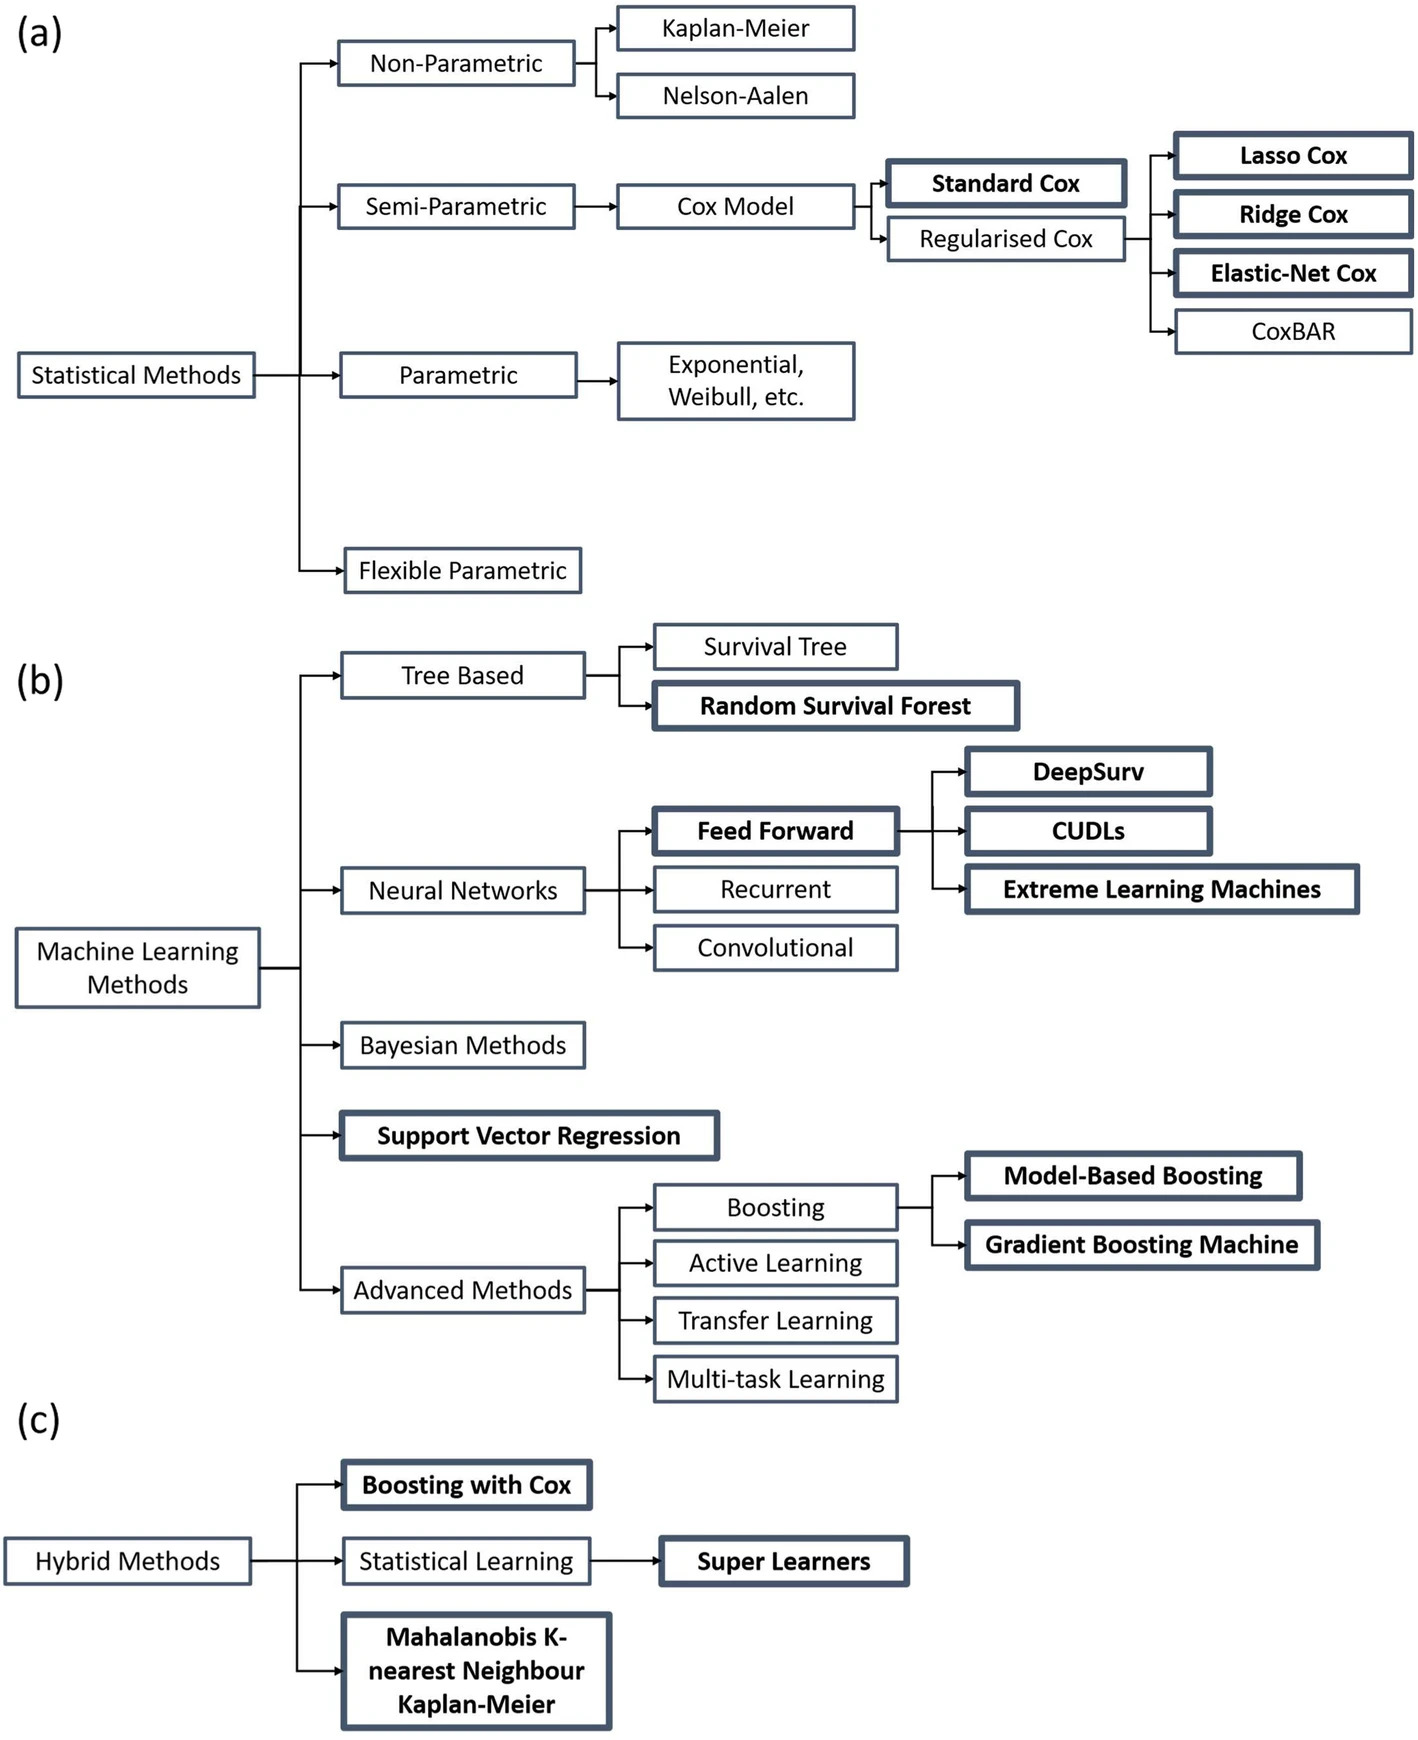
\includegraphics[scale=0.3]{Figures/ML_STATS_MODELS.jpg}
    \caption{Shows the breakdown of methods analysis preformed by \parencite{smith_scoping_2022} during a method review. The Study ran a literature selection process based on qualitative and quantitative metrics of methodology used in studies.}
    \label{fig:statsmodels}
\end{figure}

\pagebreak
\noindent Simulation studies are a crucial statistical tool used for evaluating and comparing different statistical methods, particularly when analytic solutions are hard or impossible to achieve \parencite{morris_using_2019}. These studies generate data through pseudo-random sampling from known probability distributions, enabling researchers to empirically test the behavior of statistical methods under varied scenarios. Common uses include validating new statistical methods, ensuring accuracy in mathematical models and code, and comparing the effectiveness of various approaches.
\\\\
\noindent Particularly in medical statistics, simulation studies help in designing experiments, determining sample sizes, and estimating power under specific assumptions about data generation \parencite{morris_using_2019}. Despite their widespread use, many statisticians face challenges in properly conducting simulation studies due to a lack of understanding and experience \parencite{morris_using_2019}. 
\\\\
\noindent With this research I present a comprehensive comparative study pipeline of the survival models applied to simulated survival data, highlighting their operations, challenges, and implications.

% \noindent Pinball loss \parencite{yanagisawa_proper_2023} provides a mechanism for quantile forecasting, which is particularly useful for estimating conditional quantiles of the event time distribution. The loss function is symmetric, which allows different penalties for underestimations and overestimations.
% \begin{equation} \label{eq:pinball}
% {\text{Pinball}}(\hat{F}, y; \tau) = \begin{cases} 
% (1-\tau)(\hat{F}^{-1}(\tau) - y) & \text{if } \hat{F}^{-1}(\tau) \geq y \\
% \tau(y - \hat{F}^{-1}(\tau)) & \text{if } \hat{F}^{-1}(\tau) < y 
% \end{cases}
% \end{equation}


\section{Problem Statement}
\noindent Many studies have compared machine learning with traditional statistics, yet comprehensive simulation-based comparisons are scarce. This gap may lead to biases and sometimes questionable practices, affecting the validity of findings.

\section{Research Aims and Objectives}
\subsection{Research Aims}
\noindent Perform a comparative analysis of survival models using both simulated and real datasets to identify model robustness and effectiveness, adhering to formal frameworks \parencite{morris_using_2019} and avoiding common pitfalls outlined in the literature \parencite{pawel_pitfalls_2024}.
\subsection{Objectives}
\begin{enumerate}
    \item Source a Practical Dataset: Acquire a dataset with clear constraints and features with relevant survival data. This dataset should comply with standards \parencite{wilkinson_fair_2016}. 
    \item Run the comparative study for the survival models while adhering to the ADMEP design \parencite{morris_using_2019}
    \begin{enumerate}
        \item Apply Data Generating Methods: Utilise standard libraries to generate simulated data that closely replicate the statistical properties of the real dataset.
        \item Random Survival Forest Model: Develop and apply this model using both the real and simulated datasets.
        \item Lasso Regularized Cox Proportional Hazards Model: Similarly, develop and apply this model with both datasets.
        \item Evaluate and Visualise Predictions: Use common survival analysis metrics for evaluation and employ visualization tools from survival libraries to illustrate the results effectively.
    \end{enumerate}
\end{enumerate}
 
\section{Limitations}
\begin{enumerate}
    \item \textbf{Innovation vs. Application:} This research does not venture to innovate on the algorithmic core of these methods. The primary focus is on the application and evaluation of established survival analysis methods and their existing extensions as documented in the literature. I seek to implement and test these pre-existing models in a new dataset context, thereby contributing to empirical evidence and practical applications rather than theoretical advancements.
    \item \textbf{Redundancy in Literature:} Furthermore, comprehensive comparative studies like those conducted by, \parencite{kurt_omurlu_comparisons_2009} \parencite{smith_scoping_2022} have already evaluated these methods extensively. These studies provide a solid foundation of knowledge regarding the performance and limitations of traditional and modified survival analysis models across various types of data.
\end{enumerate}

\section{Overview}
\noindent
In addressing the noted shortcomings in comparative simulation studies, this literature review methodically examines simulation work in segments relevant to each section of the study. I begin with an overview of the Cox method and its various extensions, illustrating how these foundational techniques are implemented. Following that, I explore proofs and extensions of the Lasso method, which builds on the base Cox method, enhancing its predictive power and flexibility. The discussion then moves to Random Survival Forests (RSF), detailing recent advancements in RSF algorithms that provide a solid reference for current implementations. Two comparative studies are highlighted; these utilize simulations to evaluate the methods mentioned above, offering insights into their practical applications and effectiveness. Finally, the last sections categorize the literature into subgroups that align with the specific components of the proposed research framework \parencite{pawel_pitfalls_2024} \parencite{morris_using_2019}, facilitating easy reference and integration into the research design and methodology in Chapter 2, ensuring a coherent and structured approach to applying these methods in this proposed study.

\chapter{Research Methodology}
\label{Chapter2} % For referencing this chapter elsewhere, use \ref{Chapter3}

\section{Research design} \label{design}

\noindent In this I look at the structural foundation for running the comparative study of the Random Survival Forest \parencite{ishwaran_random_2008} and the Cox proportional hazards model \parencite{cox_regression_1972}. Central to this design is the use of \textbf{simulation studies}, to gain empirical insights into the behavior of the statistical methods across various scenarios. As \parencite{morris_using_2019} aptly puts it, "Simulation studies are used to obtain empirical results about the behavior of statistical methods in certain scenarios, as opposed to analytic results."
\\\\
\noindent This section focuses on the application of the (ADMEP) framework, formalized by \parencite{morris_using_2019}. This framework is the building block of most of the methodical parts later on in the methodology. It served as the backbone of my methodology, allowing me to produce results that "accurately" reflect the performance and effectiveness of these models.

\begin{figure}[h]
 \centering
 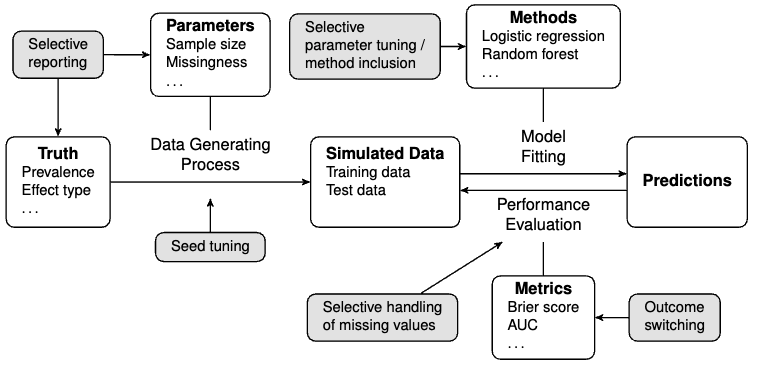
\includegraphics[scale=0.25]{Figures/METHOD_GRAPH.png}
 \caption{\parencite{pawel_pitfalls_2024} Shows a common example of a simulation study plan.}
\end{figure}

\noindent Taking inspiration from the the application of ADMEP by \parencite{pawel_pitfalls_2024}, the following sections define methods relevant in each section of the framework for later use in the methodology:

\subsection{Aims}
\begin{itemize}
\item To evaluate how effectively the Random Survival Forest and Lasso-Cox models predict survival outcomes.
\item To understand model behavior under varying conditions of data complexity and censoring rates.
\item Document research practices when conducting this study.
\end{itemize}

\subsection{Data-generating mechanisms}
\begin{itemize}
\item Simulate datasets with packages like \parencite{davidson-pilon_lifelines_2024} to introduce complexities like varying censoring rates and non-linear effects.
\item Introduce multicollinearity and various interaction effects to challenge the models' assumptions and robustness.
\end{itemize}
\
\subsubsection*{Missing Data Imputation}

As discussed in \ref{impute} we look at the methods for producing missing value imputation under the CAR and CNAR assumptions.
\\\\
\textit{Delta-adjusted Method} \parencite{jin_imputation_2024}
\begin{equation} \label{eq:deltaadjust}\lambda_{post}(t|Z_{i},X_{i}(t)) = \lambda_{\emptyset}(t|Z_{i},X_{i}(t)) = \lambda_{0}(t)\exp^{(1-\emptyset)\beta Z_{i} + \alpha X_{i}(t)}, t>C_{i}\end{equation}
\noindent The sensitivity parameter (\(\emptyset\)) represents a discounted proportion of the log-hazard ration \(\beta\) under the CNAR assumption. The method assumes that the hazard of having an event for censored subjects is multiplicatively decreased by a factor depending on the \(\emptyset\). The term \((1- \emptyset)\beta\) suggests a reduced effect of the treatment on the hazard rate post-censoring.
\\\\
\textit{Tipping point Analysis} \parencite{jin_imputation_2024}
\par \noindent This method is used to identify how much the assumption of noninformative censoring (CAR) would need to be violated for the study results to become statistically nonsignificant. It uses the delta-adjusted method's parameter \(\emptyset\) to calculate the minimum shift in \(\beta\) (log HR) needed to nullify the treatment effect.
\\\\
\textit{Jump to Reference} \parencite{jin_imputation_2024}
\begin{equation} \label{eq:jtor}\lambda_{post}(t|Z_{i},X_{i}(t)) = \lambda_{J2R}(t|Z_{i},X_{i}(t)) = \lambda_{ref}(t|X_{i}(t)) = \lambda_{0}(t)\exp^{\alpha X_{i}(t)}, t>C_{i}\end{equation}
\noindent This Method assumes that once censored, the hazard rate for a subject from the treatment group immediately aligns with that of the reference group, completely disregarding any residual effects of the treatment past the point of censoring.
\\\\
\textit{Copy Reference} \parencite{jin_imputation_2024}
\begin{equation} \label{eq:copyref}\lambda_{CR}(t|Z_{i} = 1,X_{i}(t)) = \lambda(t|Z_{i} = 0, X_{i}(t)) = \lambda_{0}(t)\exp^{\alpha X_{i}(t)} \text{for all}, t\end{equation}
\noindent This method is conservative but less so than J2R in that it assumes that if a subject in the treatment group is censored, their hazard function matches that of the reference group for the remainder of the study. It does not account for any time-specific variations in hazard that might have been influenced by the treatment before censoring.
\\\\
\textit{Censored at Random (CAR)} \parencite{jin_imputation_2024}
\par \noindent Assumes noninformative censoring where the post-censoring hazard (\(\lambda_{post}\)) is identical to the pre-censoring hazard, simplifying the imputation process.

Hazard post CAR: 
\begin{equation} \label{eq:carassmp}\lambda_{post}(t|Z_{i},X_{i}(t)) = \lambda_{0}(t)\exp^{\beta Z_{i} + \alpha X_{i}(t)}, t>C_{i}\end{equation}

Hazard post CNAR:
\begin{equation} \label{eq:cnarassmp}\lambda_{post}(t|Z_{i},X_{i}(t)) \neq \lambda_{0}(t)\exp^{\beta Z_{i} + \alpha X_{i}(t)}, t>C_{i}\end{equation}

\subsubsection*{Data Simulation}
\textit{Parametric Distribution}
\par \noindent This method is used to simulate survival times using predefined parametric distributions. The fit of each distribution to the data is tested using the one-sample Cramér-von Mises (CVM) test \parencite{thurow_how_2023}. The distribution that shows the least deviation from the data (highest p-value in the CVM test) is chosen for simulation. Parameters for these distributions are estimated using Maximum Likelihood Estimation (MLE). An Example of mixed distribution: 
\begin{equation} \label{eq:paramdist}f(x)=0.2.f_{Weibull}(\alpha,\lambda)+0.8.f_{norm}(\mu,\sigma)(x)\end{equation}
\noindent Where \(f_{Weibull(\alpha, \lambda)}\) and \(f_{norm}(\mu,\sigma)\) are the density functions for the Weibull and normal distributions, respectively.
\\\\
\textit{Kernel Density Estimation (KDE)}
\par \noindent Used to estimate by utilizing the density function of the data for simulation. The density function is estimated using the kdensity function from the \parencite{thurow_how_2023} R-package, which employs a Gaussian kernel. The Accept-reject method is used to generate random values that follow the estimated density function. Draw \((X, U)\) from the joint distribution \((X, U) ~ \left\{ (x,u):0<u<f(x)\right\}\) where X is a random variable following the estimated density f, and U is uniformly distributed between 0 and \(f(x)\). If \(u_{i} < f(x_{i})\) for a sampled \((X,U),x_{i}\) is accepted as a realization from the density function \(f\)
\\\\
\textit{Case Resampling}
\par \noindent Simulate data by resampling observed data points with replacement. Directly resample observations (ti, di) from the existing dataset of observed times and censoring indicators. \((t_{i}, d_{i})^{*}\) are drawn with replacement from \(\left\{ (t_{1}, d_{1}) \dots (t_{n}, d_{n})\right\}\)
\\\\
\textit{Conditional Bootstrapping}
\par \noindent To simulate data using bootstrapping that accounts for censoring, this helps sample censor times. For censored observations, censoring times are carried over to the simulated data. For uncensored observations, new censoring times are sampled based on the conditional distribution of censoring times given they are greater than the observed event time. Censoring Time for censored data: \(c_{i}^{*} = t_{i}\) for censored observation. Censoring Time for uncensored data: \(c_{i}^{*}\) is sampled from \(G_{i}(c) = \frac{G(c)-G(t_{i})}{1-G(t_{i})}\) where \(G\) is the distribution function of censoring times and \(t_{i}\) is the observed event time. Event times \(t^{*}_{oi}\) are sampled from the observed event times with replacement. \parencite{thurow_how_2023} Show that the reconstruction of reliable benchmark data sets is meticulously reconstructed from published Kaplan-Meier plots and other vital statistics like hazard ratios and p-values from log-rank tests. The data sets, particularly those with non-crossing survival curves, demonstrate high fidelity to the original data, proving them to be excellent resources for subsequent model evaluations.
\subsubsection*{Synthetic Data Generation}
\noindent \parencite{norcliffe_survivalgan_2023} Employ several metrics to assess synthetic survival data according to the real dataset. They help identify and correct biases in synthetic data to better align with real-world data, enhancing the credibility of survival analysis models. The optimism metric assesses whether the synthetic data is over-optimistic or over-pessimistic compared to real data by comparing the expected lifetimes derived from Kaplan-Meier (KM) plots.
\begin{equation} \label{eq:optimisim}\text{Optimism} = \frac{1}{T} \int_{0}^{T}(S_{Syn}(t)-S_{Real}(t))dt\end{equation}
\noindent Where \(S_{Syn}(t) and S_{Real}(t)\) are the synthetic and real Kaplan-Meier survival functions respectively, and T is the latest time point available. The optimism metric ranges between -1 and 1, where values closer to 0 indicate accurate lifetime predictions, positive values suggest over-optimism, and negative values indicate over-pessimism. The short-sightedness metric quantifies how much earlier synthetic data, discontinues providing predictions compared to real data, reflecting potential censorship in the synthetic modeling.
\begin{equation} \label{eq:ssmetric}\text{Short-Sightedness} = \frac{T_{Real}-T_{Syn}}{T_{Real}}\end{equation}
\noindent Here, \(T_{Syn} and T_{Real}\) are the end times of the synthetic and real Kaplan-Meier plots, respectively. This metric ranges from 0 to 1, where 0 indicates no censorship issues and 1 indicates complete short-sightedness in the synthetic data predictions. Lastly, the Kaplan-Meier divergence measures the overall divergence between the synthetic and real KM curves across the observed time, providing a comprehensive measure of similarity between the two datasets.
\begin{equation} \label{eq:kmdiverge}\text{KM Divergence} = \frac{1}{T}\int_{0}^{T}|S_{Syn}(t)-S_{Real}(t)|dt\end{equation}
\noindent This formula calculates the mean absolute difference between the synthetic and real survival functions over time, scaled by the total duration observed. The KM divergence values range from 0 to 1, where 0 indicates perfect matching KM curves and 1 represents the maximum possible difference.

\subsection{Methods}
\begin{itemize}
\item Random Survival Forest: Implement using a combination of proposed packages in \ref{methods}, tuning tree-related parameters.
\item Lasso-Cox Model: Use a combination of the proposed packages in \ref{methods} for implementing Cox regression with Lasso regularization, optimizing the regularization strength and model complexity. 
\item Explore integration effects from the different packages.
\end{itemize}

\subsubsection*{Cox Proportional Hazards Model}
The proposition consists of covariates, known as attributes regarding a unit in a distribution of data, which is associated with a coefficient \(\beta\) scaling the impact of said covariates; this product is then bound by the baseline hazard \(h_{0}(t)\).
\begin{equation} \label{eq:cox}h(t|X) = h_0(t) \exp(\beta_1 X_1 + \beta_2 X_2 + \ldots + \beta_n X_n)\end{equation}
An assumption of the Cox model is the proportional hazards assumption, suggesting that the hazard ratios for different covariates remain constant over time we see this for two events observations. This is an operational Assumption and a limitation as this is not always true for survival data. 
\begin{equation} \label{eq:coxph}\frac{h(t|X_1)}{h(t|X_2)} = \frac{h_0(t) \exp(\beta^T X_1)}{h_0(t) \exp(\beta^T X_2)} = \frac{\exp(\beta^T X_1)}{\exp(\beta^T X_2)} = \exp(\beta^T (X_1 - X_2))\end{equation}
The model can handle censoring, by adjusting the likelihood function for observations where event occurrence did not happen in a particular continuous time frame, and by maximizing the likelihood of all observed events, it is possible to estimate the coefficients that could work the best under the Cox formulation.
\begin{equation} \label{eq:coxlikely}L(\beta) = \prod_{i: \delta_i = 1} \frac{\exp(\beta^T X_i)}{\sum_{j \in R(t_i)} \exp(\beta^T X_j)}\end{equation}

\subsubsection*{Lasso Regularisation}
\noindent The Lasso technique \parencite{tibshirani_regression_1996}, a regression analysis method introduced to address specific limitations of Ordinary Least Squares (OLS) estimation, is particularly beneficial in scenarios with a large number of predictors or high collinearity among them which would mean that models could produce inflated variance scores, and cause impaired interpretability. Lasso optimizes prediction accuracy and enhances model interpretability by employing a shrinkage process that can set certain coefficients to zero effectively, thus performing variable selection.
\begin{equation} \label{eq:lasso}\hat{\beta}^{lasso} = \arg \min_{\beta} \left\{ \frac{1}{2N} \sum_{i=1}^{N} (y_i - \beta_0 - \sum_{j=1}^{p} X_{ij}\beta_j)^2 \right\}\end{equation}
bound by,
\begin{equation} \label{eq:lassobound}\sum_{j=1}^{p} |\beta_j| \leq t.\end{equation}
\noindent \parencite{freijeirogonzalez_critical_2022} The inclusion of the regularisation term, is crucial as it allows for the reduction of model complexity by penalizing the magnitude of the coefficients, which promotes sparser models. This sparsity is instrumental in enhancing interpretability by isolating only the most significant predictors that contribute to the dependent variable. The objective function of LASSO is convex for \(l_{1}\) norm, which simplifies finding the global minimum. Multiple optimal solutions might exist, especially when the number of predictors \(p\) exceeds the number of observations \(n\). \parencite{freijeirogonzalez_critical_2022} LASSO introduces bias in the coefficients to achieve lower variance and better model parsimony. Consistent under conditions like the irrepresentable condition, crucial for variable selection. Bias Correction achieved via,
\begin{equation} \label{eq:lassobais}\hat{\beta}_{j}^{LASSO}=sign(\hat{\beta}_{j}^{OLS})(|\hat{\beta}_{j}^{OLS}| - \lambda)_{+}\end{equation}

\subsubsection*{Random Survival Forest}
\noindent Random survival forests \parencite{ishwaran_random_2008} are an extension of random forests, which can handle right-censored data and aim to estimate the appropriate survival function. Consisting of an ensemble of trees \parencite{ishwaran_random_2008}, which are grown from a bootstrap sample, and each node of underlying trees, consists of specific covariates due to a random selection of features for splits in each tree.
\\\\
\noindent Per node splitting criteria are conditional to survival time and censoring, whereby node “impurity” \parencite{ishwaran_random_2008} is determined by the survival differences. Methods like log-rank, conservation of events splitting rule, and random log-rank are used. Terminal nodes are the result of saturated splitting criteria, with each endpoint having d-dimensional covariates of the individuals encapsulated. 
\\\\
\noindent A key component of the model is the conservation of events principle, which is used to define a type of predicted outcome, namely ensemble mortality, which is derived from the cumulative hazard function (CHF) using the Nelson-Aalen estimator in the original paper by \parencite{ishwaran_random_2008}. 
\\\\
\noindent Terminal nodes or nodes at the end of tree branches all share the estimated hazard function. Another key concept is the out-of-bag (OOB) samples which act as a validation subset \parencite{ishwaran_random_2008}. 
\\\\
\noindent The OOB error is calculated on the ensemble survival function of the observed data using metrics like concordance (C-index). Used for estimating prediction error and model performance without a separate test data set. Each tree's error is calculated using data not included in its training set (out-of-bag). Prediction error metrics, like the concordance index which calculates the permissible pairs per node and OOB prediction error, are used for accuracy metrics. 

\begin{equation} \label{eq:ooberror}
\hat{\Lambda}_{oob}(t,x_{i}) = \frac{1}{\sum_{b=1}^{B}I(x_{i}\in L^{b}_{oob})}\sum_{b=1}^{B}I(x_{i}\in L^{b}_{oob})\hat{\Lambda}_{b}(t,x_{i})
\end{equation}


\subsection{Estimands}
\begin{itemize}
\item Focus on estimations, like survival functions, hazard ratios, etc. for both models and survival probabilities at specified time points.
\item Bootstrap samples to build confidence intervals for key estimands, ensuring the robustness of the findings.
\item Analyze feature importance in RSF and assess how Lasso regularization affects the selection of covariates in the Cox model.
\end{itemize}

\subsubsection*{Lasso Penalised Cox Proportional Hazards}
The log partial likelihood for the Cox model, as given by:

\begin{equation} \label{eq:likelihood}l(\beta) = \sum_{i:\delta_{i}=1} \left[ \beta^{T}x_{i} - \log{\sum_{j:t_{j}\ge t_{i}} \exp(\beta^{T}x_{j})} \right]\end{equation}

\noindent Which provides a measure of how well the model's predicted hazards match the observed data. Here, \(\delta\) indicates whether an event (e.g., failure, death) was observed at time \(t_{i}\). 

\subsubsection*{Random Survival Forests}
Random forests are adapted for survival analysis by modifying how predictions are aggregated to handle censored data effectively. Forest survival function estimator:
\begin{equation} \label{eq:rsfestimator}\hat{\Lambda}(t, x_{0}) = \frac{1}{B} \sum_{b=1}^{B} \hat{\Lambda}_{b}(t,x_{0})\end{equation}
Survival function:
\begin{equation} \label{eq:survrsf}S(t,x_{0}) = \exp^{-\hat{\Lambda}(t,x_{0})}\end{equation}

\noindent Variable importance (VI) \parencite{pham_springer_2023} in random forests is used to rank variables based on their contribution to prediction accuracy. It is assessed by looking at each predictor variable in the sample and assessing the impact on prediction error, an increase in error indicating importance. Different random forest settings can yield different importance rankings due to the model's sensitivity to the configuration. VI is shown by \parencite{pham_springer_2023}:
\begin{equation} \label{eq:vinorm}
VI(j) = \frac{1}{B}\sum_{b=1}^{B}(\frac{Err(j)_{b}}{Err_{b}}-1)
\end{equation}

\noindent VI Adaptation:
\begin{equation} \label{eq:viadapt}VI(j) = \frac{1}{B}\sum_{b=1}^{B}(\frac{Err(j|Z)_{b}}{Err_{b}}-1)\end{equation}

\noindent This adaptation \ref{eq:viadapt} addresses correlations \parencite{pham_springer_2023} by conditioning on other related variables. This accounts for the influence of correlated predictors by adjusting the variable importance calculation.


\subsection{Performance measures}
\begin{itemize}
\item Use statistical tests, like the C-index, and integrated Brier score to compare the RSF and Lasso-Cox model's performance metrics, like predictive accuracy, discrimination, and calibration across time.
\item Conduct sensitivity analysis to explore the impact of model parameters on their performance.
\item Apply graphical methods like Kaplan-Meier curves to visualize survival estimates against actual outcomes.
\end{itemize}

\subsubsection*{C-Index}
\noindent The C-index \parencite{qi_effective_2023}, serves as a crucial statistical measure in evaluating the effectiveness of survival models. This index assesses how well these models predict the sequence of patient outcomes based on their respective risk assessments. It is defined as the ratio of pairs of subjects (deemed "comparable") for which the model's predictions and actual outcomes are consistent in terms of event sequence. "Comparable" refers to pairs where the event sequence, i.e., who encountered the event first, can be established.
\begin{equation} \label{eq:cindex}C\text{-index} = \frac{\sum_{i,j} \mathbf{1}(t_i < t_j) \cdot \mathbf{1}(\eta_i > \eta_j) \cdot \delta_i}{\sum_{i,j} \mathbf{1}(t_i < t_j) \cdot \delta_i}\end{equation}
\noindent In this formula, \(\mu_{i}\) is the risk score for unit i, and \(\delta_{i}\) indicates whether an event occurred (1 if it did, 0 otherwise)
\subsubsection*{Brier Score and Integrated Brier Score}
\textit{Brier score} is a measure used to evaluate the accuracy of probabilistic predictions. It is essentially the mean squared error \parencite{qi_effective_2023} between the observed outcomes and the predicted probabilities at a specific time \(t^{*}\).
\begin{equation} \label{eq:bs}BS_{t^*}(VU, \hat{S}(t^* | \cdot)) = \frac{1}{|VU|} \sum_{[\tilde{x}_i, d_i] \in VU} (I[d_i \leq t^*] - \hat{S}(t^* | \tilde{x}_i))^2\end{equation}
\noindent Where, \(VU\) is the validation set, \(\hat{S}(t^* | \cdot))\) is the predicted survival probability at \(t^{*}\) and \(I[d_i \leq t^*]\) is the event indicator.
\\\\
\noindent \textit{Integrated Brier Score (IBS)} extends the Brier score across a range of times, providing a measure of model accuracy over time. In other words, it is the expectation of the Brier scores calculated at each time point within a specified interval.
\begin{equation} \label{eq:ibs}IBS(\tau, VU, \hat{S}(\cdot | \cdot)) = \frac{1}{\tau} \int_0^{\tau} BS_t(VU, \hat{S}(t | \cdot)) \, dt\end{equation}
\noindent Where, \(\tau\) is the biggest event period, \(BS_{t}\) is the brier score at time t.
\subsubsection*{1-Calibration}
\noindent 1-Calibration, also known as Hosmer-Lemeshow calibration, is a test used to evaluate model calibration at a specific time point \(t^{*}\) \parencite{haider_effective_2018}.
It works by sorting all subjects for the predicted probabilities at time \(t^{*}\). These probabilities are then grouped into a predefined number of groups or bins (typically 10). For each bin, number of events is determined based on the predicted probabilities, and this is compared to the actual number of events that occurred \parencite{qi_effective_2023}.

\begin{equation} \label{eq:c1}\text{HL}(VU, \hat{S}(t^* | \cdot)) = \sum_{j=1}^B \frac{(O_j - n_j \bar{p}_j)^2}{n_j \bar{p}_j (1 - \bar{p}_j)}\end{equation}
\noindent Where, \(B\) is the number of bins, \(O_{j}\) is the observed number of events in bin j, \(\hat{p}_{j}\) is the average predicted probability in bin j. 

\subsubsection*{D-Calibration}
\noindent D-Calibration \parencite{haider_effective_2018} extends the concept of 1-calibration over a range of time points or across different distributions of time points, providing a more comprehensive measure of a model's accuracy.

% \begin{equation} \label{eq:dc}D_{\Theta}([a, b]) = \{[x_i, d_i, \delta_i = 1] \in D | \hat{S}_{\Theta}(d_i) \in [a, b]\}\end{equation}

\subsubsection*{Mean Absolute Error}
\par \noindent \textit{Mean Absolute Error} (MAE) (Uncensored) is the simplest form of MAE variants indicated by \parencite{qi_effective_2023}, it is calculated by taking the non negative value difference between the predicted and actual event times for uncensored subjects only. It does not consider censored data, which may introduce bias when censoring rate is frequent.
\begin{equation} \label{eq:rmae}
RMAE (\hat{t}_i, t_i, \delta_i = 1) = |t_i - \hat{t}_i|
\end{equation}
\par \noindent \textit{MAE-Hinge} variant \parencite{qi_effective_2023} considers only the cases where the estimated time is sooner than the actual cesonsoring time. It is somewhat optimistic as it assigns zero error to predictions that are later than or equal to the censoring time. Applied when the actual event time is censored \(\delta (i =0)\)
% \begin{equation} \label{eq:maehinge}
% RMAE\text{-hinge}(\hat{t}_i, t_i, \delta_i = 0) = \max(t_i - \hat{t}_i, 0)
% \end{equation}
\par \noindent \textit{"MAE-Margin"} \parencite{qi_effective_2023} uses a "margin time" for induvivual censored units, estimated using a non-parametric method (Kaplan-Meier estimator). This "margin time" is treated as an adjusted event time, creating a more informed guess for censored individuals.
\begin{equation} \label{eq:maemargin}
\text{Error for censored subjects:} \quad \omega_i[(1 - \delta_i) \cdot \text{emargin}(t_i) + \delta_i \cdot t_i] - \hat{t}_i
\end{equation}
\noindent \parencite{qi_effective_2023} shows that \(w_{i} = 1-S_{KM}(t_{i})\) confidence weight based on the Kaplan-Meier estimator \(emargin(t_{i})=t_{i}+\int_{t_{i}}^{\infty} S_{KM}(D)(t)/S_{KM}(D)(t_{i})\) margin time.
\\\\
\noindent \textit{"MAE-IPCW-D"} ("Inverse Probability Censoring Weight" - Difference) adapts the "IPCW" method to MAE by re-allocating the weights of censored subjects to those with known outcomes, using the estimated time of the event for calculations.
\par \noindent Then, \textit{RMAE-IPCW-T} is calculated similarly to RMAE-IPCW-D, but using eIPCW  for censored subjects. MAE-PO (Pseudo-Observation) utilizes pseudo-observations that estimate the impact of each data point on the overall survival time estimate. 
\begin{equation} \label{eq:maepsuedo}e_{pseudo-obs}(t_i, D) = N \cdot \hat{\theta} - (N - 1) \cdot \hat{\theta}_{-i}\end{equation}
\par \noindent \(\theta\) and \(\hat{\theta}\) are unbiased survival time estimators with and without the ii-th subject. The pseudo-observation is treated as an observed event time for MAE calculations.

% \subsubsection*{Ranked Probability Score}
% Ranked probability score \parencite{yanagisawa_proper_2023} extends the concept of the Brier Score to multi-class problems by considering the cumulative probability distributions. It evaluates the accuracy of predictions across all possible categorical outcomes, making it highly useful for discrete classification tasks in survival analysis.
% \begin{equation} \label{eq:ranked}S_{\text{RPS}}(\hat{F}, y) = \sum_{i=1}^{B-1} S_{\text{Binary-Brier}}(\hat{F}, y; \zeta_i)\end{equation}

\subsubsection*{Logarithmic Score}
The Logarithmic Score \parencite{yanagisawa_proper_2023} is used for models that predict the entire probability distribution of the event times. It rewards models that assign higher probabilities to the events that occur. It assesses the logarithm of the predicted probabilities assigned to the true outcome intervals, promoting models that are confident and correct about their predictions.
\begin{equation} \label{eq:logscore}S_{\text{Log}}(\hat{F}, y; \{\zeta_i\}) = -\sum_{i=0}^{B-1} 1(\zeta_i < y \leq \zeta_{i+1}) \log(\hat{F}(\zeta_{i+1}) - \hat{F}(\zeta_i))\end{equation}

\subsubsection*{Cross-Validation}
\parencite{harrell__regression_2015} Cross-validation is a resampling technique used to evaluate the generalizability of a statistical model by systematically partitioning the dataset into training and validation subsets. The most granular form, leave-one-out cross-validation (LOOCV), omits one observation at a time from the dataset of size $n$, fits the model on the remaining $n-1$ observations, and uses the excluded observation to test the model's performance. The process is repeated $n$ times, yielding an average accuracy metric, typically denoted by $\hat{\theta} = \frac{1}{n} \sum_{i=1}^{n} \theta_i$, where $\theta_i$ is the performance metric for the $i$-th iteration. Grouped cross-validation, a more practical alternative, divides the data into $k$ subsets, using $k-1$ subsets for model training and the remaining subset for validation, iterating this process $k$ times. Although cross-validation mitigates some issues of data-splitting, it is computationally expensive, often requiring numerous repetitions (e.g., 200+ iterations) to stabilize accuracy estimates. Moreover, the method may not fully capture the variability of variable selection, as subsets tend to produce similar feature sets. Additionally, cross-validation does not validate the model on the full dataset, which can lead to an underestimation of the model's overall predictive power. To address potential overfitting, a randomization method can be employed, where the response variable $Y$ is randomly permuted, and the model's predictive accuracy on this randomized data is compared to its performance on the original data, with significant deviations indicating possible overfitting.

\section{Data}
\noindent For my research, I utilized SurvSet, an open-source repository specifically designed for time-to-event (T2E) analysis. SurvSet provides a standardized collection of 76 datasets, primarily focused on biomedicine, that are formatted consistently for easy preprocessing and analysis. This makes it an ideal source for benchmarking machine learning (ML) algorithms in survival analysis.
\\\\
\noindent To understand the specifics of each dataset within SurvSet, the repository provides a clear and consistent structure. Each dataset is accompanied by a unique ds\_name and metadata that detail its characteristics, such as whether it includes time-dependent covariates, the number of features, and the types of variables (numerical or categorical). The SurvLoader class allows users to easily load any dataset and access this metadata, along with a reference URL that offers additional context and explanations for the columns. This structure ensures that researchers can quickly grasp what each dataset is used for and how it can be applied in survival analysis or machine learning benchmarking.
\\\\
\noindent SurvSet organizes datasets using a SurvLoader class, which simplifies loading and accessing data. Each dataset includes core columns like \texttt{pid} (unique ID), \texttt{event} (whether the event occurred), and \texttt{time} (time to event or censoring). Features are clearly marked as either numerical (num\_\{\}) or categorical (fac\_\{\}), ensuring a smooth integration with various ML algorithms. This consistent structure across all datasets in SurvSet made it my go-to source for accurate and reliable survival analysis in my project.
\\\\
\noindent Furthermore, when selecting the dataset censoring levels, FAIR principles \parencite{wilkinson_fair_2016}, reproducibility by assessing data simulation accuracy similar to the KM-Divergence metric used by \parencite{norcliffe_survivalgan_2023} are all important considerations. Utilizing this approach voids the need to carefully assess the ethical implications of using the datasets as these datasets should be under public licensed availability. Lastly, I don't foresee data preprocessing steps, being necessary, as DGM for simulation are commonly categorized as postprocessing \parencite{jin_imputation_2024}.


\section{Methods} \label{methods}
\subsection{Exploratory Analysis}
Exploratory Data Analysis (EDA) is a crucial first step to discover key considerations for contributing covariates and potential implications. In line with the principles outlined in \parencite{harrell__regression_2015}, this EDA focuses on a detailed examination of the survival data's structure, distribution, and key features such as outliers, missing values, and multicollinearity, that could impact the performance and validity of our regression models.
\\\\
\noindent \textit{Data Overview} The dataset's dimensions, including the number of rows and columns, are first examined to understand its size. Next, we verify the data types of each column (such as time, event, and covariates) to ensure they are appropriate for analysis. Additionally, we identify and assess missing values across the dataset, visualizing these patterns using a heatmap or matrix plot to uncover any systematic issues.
\\\\
\noindent \textit{Target Variable Analysis (Survival Time and Event Status)} For the survival time (time), summary statistics such as mean, median, range, and standard deviation are calculated. We then plot the distribution of survival times using a histogram or density plot to visualize these statistics. For the event status (event), the proportion of events versus censored cases is determined and visualized through a bar chart to understand the distribution of event occurrences.
\\\\
\noindent \textit{Univariate Analysis of Covariates} In the univariate analysis, summary statistics for each numerical covariate are calculated, including the mean, median, minimum, and maximum values. These statistics are further visualized through histograms or density plots to assess their distributions. For categorical covariates, we count the frequency of each category and visualize the distribution using bar charts.
\\\\
\noindent \textit{Bivariate Analysis} To explore relationships between survival time and covariates, scatter plots are created for numerical covariates, while box plots are used to compare survival times across different levels of categorical covariates. For the event status versus covariates, bar charts or stacked bar charts are used to visualize the distribution of event status across categorical covariates. Violin plots or box plots are also employed to assess the distribution of numerical covariates within each event status, such as comparing values for censored versus event occurred.
\\\\
\noindent \textit{Censoring Analysis} Censoring is analyzed by calculating and visualizing the overall censoring level in the dataset, expressed as the percentage of censored observations. Additionally, we explore how censoring is distributed across different covariates by creating grouped bar charts or box plots.
\\\\
\noindent \textit{Correlation Analysis} For numerical covariates, a correlation matrix is calculated and visualized using a heatmap to identify relationships between variables. For categorical covariates, relationships with numerical covariates are explored using point-biserial correlations, while Chi-square tests are used where appropriate to examine relationships between categorical variables.

\subsection{Data Processing and Simulation}

\subsubsection*{Data Processing}
\subsubsection*{Simulation}
For the simulation, I utilized the Synthcity library \parencite{qian_synthcity_2023}. Synthcity is an open-source package designed for generating and evaluating synthetic data across various data modalities, including static data, regular and irregular time series, and censored data. It provides a unified platform for innovative use cases in machine learning fairness, privacy, and data augmentation. The library was chosen for its comprehensive support of survival analysis and synthetic data generation, making it an ideal tool for this study.
\begin{figure}[h]
    \centering
    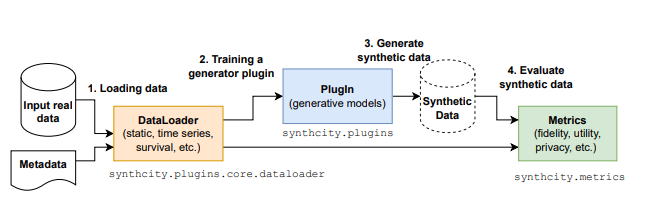
\includegraphics[scale=0.68]{Figures/SynthCity.png}
    \caption{\parencite{qian_synthcity_2023} Simulation Pipeline.}
\end{figure}

\noindent Among the various generative models available in Synthcity, I focused on the use of Survival GAN and Survival VAE. These methods were selected based on previous explorations and their proven ability to handle the complexities of survival data. Survival GAN is particularly effective in generating high-fidelity data with the capability to preserve the underlying distribution, while Survival VAE offers a robust framework for capturing the latent structure of the data, making it suitable for the simulation of censored survival datasets.
The simulation pipeline is designed to effectively generate synthetic survival data that mirrors real-world datasets, following the structured process provided by Synthcity. The design integrates several key components and classes from Synthcity, ensuring a comprehensive approach to data generation and evaluation.
\\\\
\noindent \textit{Data Loading.} \parencite{qian_synthcity_2023} The first step in the pipeline involves loading the real survival datasets using the \texttt{DataLoader} class from Synthcity. The \texttt{DataLoader} processes the survival times, censoring indicators, and covariates. Furthermore The \texttt{DataLoader} provides validation for censored observations, ensuring that the survival times and event indicators are correctly aligned for downstream modeling. Metadata, such as identifying sensitive features or specifying outcome variables, can be included.
\\\\
\noindent \textit{Model Training.} The \texttt{Plugin} class is used to instantiate these models, allowing for straightforward training and application. The training is conducted using the \texttt{fit()} method of the \texttt{Plugin} class.
\\\\
\noindent \textit{Synthetic Data Generation.} Once the models are trained, the \texttt{generate()} method of the \texttt{Plugin} class is used to produce synthetic datasets. The design considerations at this stage include:
\\\\
\noindent \textit{Evaluation of Synthetic Data.} The final component of the pipeline involves evaluating the synthetic data using the \texttt{Metrics} class provided by Synthcity. The design focuses on several key evaluation aspects:
\begin{itemize}
    \item Fidelity Metrics: The \texttt{Metrics} class is utilized to assess how closely the synthetic data resembles the original data. Metrics such as distributional similarity and survival curve alignment are critical for determining data fidelity. 
    \item Utility Evaluation: The utility of the synthetic data for downstream tasks is tested by applying standard machine learning models to the generated data and comparing performance against models trained on real data. 
    \item Privacy Considerations: Privacy is a major concern in synthetic data generation. The \texttt{Metrics} class includes tools to evaluate the privacy of the synthetic data, such as assessing the risk of re-identification or leakage of sensitive information. 
\end{itemize}

\subsection{Survival Analysis: Model Application and Evaluation}

\noindent For this section I outline the steps For running the models on the loaded and preperad data. The libraries utilized in the study consist of:

\begin{table}[h]
\begin{tabularx}{\textwidth}{|X|X|}
\hline
Library/Method & Description \\
\hline
Auton-survival \parencite{nagpal_auton-survival_2022} & Provides tools for survival analysis including implementations of advanced machine learning models like DeepSurv and Cox-Time. \\
\hline
scikit-survival \parencite{sebastian_polsterl_scikit-survival_2023} & Extends scikit-learn \parencite{scikit-learn} to handle survival analysis, enabling use of Cox regression models with extensions such as Lasso. \\
\hline
lifelines \parencite{davidson-pilon_lifelines_2024} & Popular library for survival analysis that includes Kaplan-Meier, Nelson-Aalen, and Cox models, among others. \\
\hline
\end{tabularx}
\caption{Libraries to be used during research}
\label{tab:libs}
\end{table}

\subsubsection*{Cox Proportional Hazards (CoxPH) Model}

\paragraph*{Model Fitting}
\begin{itemize}
    \item Fit the CoxPH model using the \texttt{lifelines} library.
    \item Check the proportional hazards assumption with \texttt{lifelines.check\_assumptions()}.
\end{itemize}

\paragraph*{Lasso Regularization}
\begin{itemize}
    \item Apply Lasso regularization (L1 penalty) during the fitting process to perform feature selection by shrinking coefficients of less important covariates to zero.
    \item Use the \texttt{lifelines.CoxPHFitter(penalizer=penalty)} with a chosen penalty term to control the amount of regularization applied. 
    \item Use metrics like the cross-validation score
\end{itemize}

\paragraph*{Effect of Lasso on Model Performance}
\begin{itemize}
    \item Lasso regularization can help reduce model complexity by selecting a subset of relevant covariates, which may improve the interpretability and generalization of the CoxPH model.
    \item Evaluate the impact of Lasso on model performance by comparing the concordance index (C-index) and analyzing the selected covariates.
\end{itemize}


\paragraph*{Survival Curve Prediction}
\begin{itemize}
    \item Predict survival function using \texttt{predict\_survival\_function()}.
    \item Plot survival curves for different covariate profiles.
\end{itemize}


\paragraph*{Covariate Contribution Analysis}
\begin{itemize}
    \item Use \texttt{lifelines.plot\_covariate\_groups()} to visualize covariate impact.
    \item Create boxplots to analyze covariate effects on the hazard ratio.
\end{itemize}

\paragraph*{Model Evaluation}
\begin{itemize}
    \item Compute concordance index (C-index) for model performance.
    \item Evaluate model performance across different levels of censoring.
    \item Perform stratified analysis based on different censoring levels.
    \item Validate model with cross-validation or bootstrap methods.
\end{itemize}

\paragraph*{Assumption Checking}
\begin{itemize}
    \item Validate proportional hazards assumption with Schoenfeld residuals.
    \item Explore any violations and consider adjustments like stratified models.
\end{itemize}

\subsubsection*{Random Survival Forest (RSF) Model}

\paragraph*{Model Fitting}
\begin{itemize}
    \item Fit the RSF model using a the library \texttt{scikit-survival}.
    \item Tune model parameters (e.g., number of trees, max depth).
\end{itemize}

\paragraph*{Survival Curve Prediction}
\begin{itemize}
    \item Predict survival curves for each observation.
    \item Aggregate and plot survival probabilities across different covariate profiles.
\end{itemize}

\paragraph*{Variable Importance}
\begin{itemize}
    \item Analyze covariate importance using the \texttt{variable\_importance\_} attribute.
    \item Visualize importance scores using Logarithmic plot for identifing contributers.
\end{itemize}

\paragraph*{Model Evaluation}
\begin{itemize}
    \item Evaluate model using out-of-bag (OOB) score or concordance index.
    \item Evaluate model performance across different levels of censoring.
    \item Analyze performance under different levels of censoring.
    \item Validate model with cross-validation or bootstrap methods.
\end{itemize}

\paragraph*{Comparison with CoxPH}
\begin{itemize}
    \item Compare survival curves from both models for specific covariate profiles.
    \item Analyze differences, especially in cases with high censoring or non-proportional hazards.
\end{itemize}

\subsection{Research Practice Evaluation}

The core focus of this evaluation is not to interpret the effects or outcomes of the models in detail, but rather to ensure that the research practices applied throughout the simulation study are rigorous and well-documented. By concentrating on the methodological aspects, we aim to establish a reliable foundation for the simulation without delving into the specific interpretations of model results. This approach allows us to maintain objectivity and consistency in evaluating the effectiveness and validity of the simulation pipeline.
\\\\
\noindent To achieve this, a clear labeling strategy is employed, using abstract descriptions for each subprocess within the full simulation study. This labeling strategy helps in systematically categorizing and tracking the various steps, ensuring that every component of the simulation is transparently documented. The use of abstract labels also facilitates a higher-level understanding of the simulation process, making it easier to identify potential areas for refinement and ensuring that the entire workflow remains coherent and aligned with the study’s objectives.
    

\section{Limitations} \label{methlim}
A massive limitation is that the research is tightly coupled, meaning the phases are strictly dependent on each other. This is an antipattern, \parencite{joshi_beginning_2016}, which should be planned to accommodate any failures during any of the research phases. In cases where results do not converge, or the interpretation is wrong, the tightly coupled nature of the research will also affect the preceding stages. Lastly the computation time, within the modern setting should not be a hindrance but the combination of multiple computational components like the DGM and the model execution and results evaluation, is important to take caution. 

\section{Ethical Considerations}
Ethical clearance would not be a component of this study, as the only real data that would be used, will only be selected from open source, or publicly available (public licensing) sources. Due to the nature of the topic, being closely related to sensitive information, it will be an important point of order to note in the case that results indicate or underscore ethical implications.

\chapter{Schedule of Work}
\label{Chapter3} % For referencing this chapter elsewhere, use \ref{Chapter4}


\noindent Lorem ipsum dolor sit amet, consectetur adipiscing elit. Aliquam ultricies lacinia euismod. Nam tempus risus in dolor rhoncus in interdum enim tincidunt. Donec vel nunc neque. In condimentum ullamcorper quam non consequat. Fusce sagittis tempor feugiat. 

\par\vspace{0.5cm}
\noindent \Cshadowbox{
	\begin{minipage}{15cm}
		\bigskip
		\color[rgb]{0.0,0.4,0.65}The chapter puts forward the planned schedule of work for the research. In it, you should
		this chapter, you should provide an overview and \emph{discussion} of the planned schedule for the research. Your discussion should 
		\begin{itemize}
			\item present and discuss the schedule of work,
			\item identify any foreseeable difficulties to carrying out the project according to the planned schedule,
			\item provide a brief conclusion to the chapter.
		\end{itemize} 
		\medskip
\end{minipage}}\\


\section{Schedule of Work}

Sed ullamcorper quam eu nisl interdum at interdum enim egestas. Aliquam placerat justo sed lectus lobortis ut porta nisl porttitor. Vestibulum mi dolor, lacinia molestie gravida at, tempus vitae ligula. Donec eget quam sapien, in viverra eros. Vivamus ornare ultrices facilisis. Ut hendrerit volutpat vulputate. Morbi condimentum venenatis augue, id porta ipsum vulputate in. Curabitur luctus tempus justo. Vestibulum risus lectus, adipiscing nec condimentum quis, condimentum nec nisl. Aliquam dictum sagittis velit sed iaculis. Morbi tristique augue sit amet nulla pulvinar id facilisis ligula mollis. Nam elit libero, tincidunt ut aliquam at, molestie in quam. Aenean rhoncus vehicula hendrerit. \par 
\medskip


\begin{ganttchart}[
	time slot format=isodate-yearmonth,
	time slot unit=month,
	]{2019-01}{2020-09}
	\gantttitlecalendar{year, month} \\
	\ganttgroup{Objective 1}{2019-01}{2019-11} \\
	\ganttbar{Task 1}{2019-02}{2019-08} \\
	\ganttbar{Task 2}{2019-02}{2019-11} \\
	\ganttmilestone{Milestone 1}{2019-11} \\
	\ganttgroup{Objective 2}{2019-12}{2020-08} \\
	\ganttbar{Task 3}{2019-12}{2020-08} \\
	\ganttbar{Final Task}{2020-06}{2020-08}
	\ganttlink[link type=s-s]{elem1}{elem2}
	\ganttlink[]{elem2}{elem3}
	\ganttlink[]{elem3}{elem5}	
	\ganttlink[link type=f-f]{elem5}{elem6}
	
\end{ganttchart}

\medskip

Lorem ipsum dolor sit amet, consectetur adipiscing elit. Aliquam ultricies lacinia euismod. Nam tempus risus in dolor rhoncus in interdum enim tincidunt. Donec vel nunc neque. In condimentum ullamcorper quam non consequat. Fusce sagittis tempor feugiat. Fusce magna erat, molestie eu convallis ut, tempus sed arcu. Quisque molestie, ante a tincidunt ullamcorper, sapien enim dignissim lacus, in semper nibh erat lobortis purus. Integer dapibus ligula ac risus convallis pellentesque. 

\section{Potential Difficulties}

Sed ullamcorper quam eu nisl interdum at interdum enim egestas. Aliquam placerat justo sed lectus lobortis ut porta nisl porttitor. Vestibulum mi dolor, lacinia molestie gravida at, tempus vitae ligula. Donec eget quam sapien, in viverra eros. Donec pellentesque justo a massa fringilla non vestibulum metus vestibulum. Vestibulum in orci quis felis tempor lacinia. Vivamus ornare ultrices facilisis. 



\chapter{Conclusion}
\label{Chapter4}


\noindent In this study, I explored the application of Random Survival Forests (RSF) and Cox Proportional Hazards models in survival analysis, focusing on evaluating their performance through dynamic parameter tuning and the use of synthetic data generated by Survival GAN and Survival VAE models. The simulation results demonstrated that both models provide valuable insights into the underlying patterns of the dataset, with the RSF model showing slightly improved performance in survival prediction and cumulative hazard estimates. However, the Cox model, once convergence issues were addressed through preprocessing and variable selection techniques, proved to be a robust alternative for simpler survival data structures.
\\\\
\noindent The comparison between the models revealed that while the Cox model performed well in terms of metrics like concordance and calibration, the RSF model's flexibility in handling complex interactions and high-dimensional data provided it with an edge, particularly in Brier score and integrated Brier score (IBS). Despite the computational cost associated with tuning parameters in the RSF model, the results highlight its effectiveness in survival analysis, especially when dealing with more intricate datasets.
\\\\
\noindent In addition, the exploratory data analysis (EDA) provided crucial insights into the structure of the dataset, with the correlation matrix and bivariate analysis identifying key relationships between variables, such as the skewed distribution of age and its effect on survival. The visualizations generated through the RSF and Cox models helped validate these findings, further emphasizing the importance of selecting appropriate models based on the complexity of the data.
\\\\
\noindent Ultimately, this simulationstudy underscores the value of using a robust framework like ADMEP \parencite{morris_using_2019} to easily apply advanced machine learning techniques like RSF in survival analysis, particularly in scenarios where high-dimensional data and complex variable interactions come into play. The results also suggest that model selection should be guided by both performance metrics and the computational feasibility of tuning parameters, especially in resource-constrained environments.
\\\\
\noindent The metrics employed, such as concordance, Brier score, integrated Brier score (IBS), and calibration errors, are critical for evaluating the performance of survival models across diverse datasets. By applying these metrics consistently, a fair comparison can be drawn between the Random Survival Forest (RSF) and Cox Proportional Hazards (CoxPH) models, providing a comprehensive understanding of how each model performs under various data structures \parencite{harrell__regression_2015}. This approach ensures that model evaluation is not solely based on a single dataset, which might lead to biased conclusions. Instead, it allows for generalizability across multiple datasets, capturing a wider range of complexities and ensuring that model performance is robust and adaptable to different survival scenarios \parencite{tibshirani_regression_1996}. The dynamic nature of the metrics, especially those like Brier score and IBS, further aids in understanding model behavior over time, making them more relevant for long-term predictions in survival analysis \parencite{qi_survivaleval_2024}.
\\\\
\noindent Moreover, the use of simulation models like Survival GAN and Survival VAE not only facilitates ethical clearance by circumventing the need for sensitive or limited real-world data but also allows for the introduction of controlled variance and different survival patterns \parencite{norcliffe_survivalgan_2023}. This flexibility in generating synthetic data is invaluable in survival analysis, as it enables the testing of models under various conditions, including varying degrees of censoring, time-dependent covariates, and event rates. By introducing such controlled variance, simulations provide a more rigorous testing ground for survival models, ensuring that they can handle diverse data types and scenarios before applying them to real-world datasets. This capability enhances the models' adaptability and resilience, ultimately leading to more reliable and generalizable insights across different survival analysis applications \parencite{qian_synthcity_2023}.

%----------------------------------------------------------------------------------------
%	THESIS CONTENT - APPENDICES
%----------------------------------------------------------------------------------------

% \appendix % Cue to tell LaTeX that the following "chapters" are Appendices

% Include the appendices of the thesis as separate files from the Appendices folder
% Uncomment the lines as you write the Appendices

% \chapter{Appendix Title} % Main appendix title
\label{AppendixA} % For referencing this appendix elsewhere, use \ref{AppendixA}

\section{Main Section}

\noindent Lorem ipsum dolor sit amet, consectetur adipiscing elit. Aliquam ultricies lacinia euismod. Nam tempus risus in dolor rhoncus in interdum enim tincidunt. Donec vel nunc neque. In condimentum ullamcorper quam non consequat. Fusce sagittis tempor feugiat. Fusce magna erat, molestie eu convallis ut, tempus sed arcu.

\par\vspace{0.5cm}
\noindent \Cshadowbox{
	\begin{minipage}{15cm}
		\bigskip
		\color[rgb]{0.0,0.4,0.65} The appendices are sections in which complicated mathematical or other formulae, descriptions of experiments or apparatus, and any other specialised or lengthy material such as computer programme listings, copies of spectra or other instrumental outputs are found.  
		\medskip
\end{minipage}}\\

\begin{table}[h!]
    \centering
    \begin{tabular}{|l|l|p{10cm}|}
    \hline
    \textbf{Label} & \textbf{Category} & \textbf{Description} \\ \hline
    DP   & Data Preparation (General)   & General label for all data preparation tasks, including cleaning, transformation, and preprocessing. \\ \hline
    MDH  & Missing Data Handling        & Specific tasks related to identifying, handling, and imputing missing data. \\ \hline
    ENC  & Data Encoding                & Tasks related to encoding categorical variables, feature scaling, and other data transformations. \\ \hline
    DS   & Data Splitting               & Splitting the data into training, validation, and testing sets. \\ \hline
    MI   & Model Initialization         & Initializing models with chosen parameters, including setting up cross-validation schemes. \\ \hline
    MT   & Model Training (General)     & General label for tasks related to model training, including fitting the model to training data. \\ \hline
    HT   & Hyperparameter Tuning        & Tasks focused on optimizing model parameters, such as grid search or random search. \\ \hline
    REG  & Regularization Application   & Applying regularization techniques like Lasso, Ridge, or Elastic Net during model fitting. \\ \hline
    SA   & Survival Analysis (General)  & General label for survival analysis tasks, including survival function estimation and survival curve plotting. \\ \hline
    CIA  & Covariate Impact Analysis    & Analyzing the impact of individual covariates on the outcome, including statistical tests and visualizations. \\ \hline
    ME   & Model Evaluation (General)   & General label for evaluating model performance across various metrics. \\ \hline
    CV   & Cross-Validation             & Performing cross-validation to assess model performance stability. \\ \hline
    AC   & Assumption Checking (General) & General label for checking model assumptions, including proportional hazards or other key assumptions. \\ \hline
    BVT  & Bias-Variance Tradeoff       & Analyzing the tradeoff between bias and variance in model performance. \\ \hline
    SS   & Simulation Setup             & Setting up the simulation environment, including configuring parameters and preparing input data. \\ \hline
    SDG  & Synthetic Data Generation (General) & General label for generating synthetic datasets using trained models. \\ \hline
    SDE  & Synthetic Data Evaluation (General) & General label for evaluating the quality and utility of generated synthetic data. \\ \hline
    RC   & Results Compilation          & Compiling and summarizing results from various stages of the study for reporting. \\ \hline
    DR   & Documentation and Reporting  & Documenting processes, decisions, and findings throughout the study for transparency and reproducibility. \\ \hline
    CM   & Comparison of Models         & Comparing results from different models or approaches, such as CoxPH vs. RSF. \\ \hline
    \end{tabular}
    \caption{Labeling Strategy for Simulation Study}
    \label{tab:labeling_strategy}
    \end{table}
% \chapter{Using this Template} % Main appendix title
\label{AppendixB} % For referencing this appendix elsewhere, use \ref{AppendixB}

\par\vspace{1cm}
\Cshadowbox{
	\begin{minipage}{15cm}
		\bigskip
		\color[rgb]{0.0,0.4,0.65}In the following appendix, some of the guidance from the original template is included. This includes the
			\begin{itemize}
				\item files and folders included in the template,
				\item guidance on filling the main.tex file with your information,  
				\item guidance on including references, tables, figures, and mathematical formulae.
			\end{itemize} 
		\bigskip
\end{minipage}}\\

\section{What this Template Includes}

\subsection{Folders}

This template comes as a single zip file that expands out to several files and folders. The folder names are mostly self-explanatory:

\keyword{Appendices} -- this is the folder where you put the appendices. Each appendix should go into its own separate \file{.tex} file. An example and template are included in the directory.

\keyword{Chapters} -- this is the folder where you put the thesis chapters. Each chapter should go in its own separate \file{.tex} file.

\keyword{Figures} -- this folder contains all figures for the thesis. These are the final images that will go into the thesis document.

\subsection{Files}

Included are also several files, most of them are plain text and you can see their contents in a text editor. After initial compilation, you will see that more auxiliary files are created by \LaTeX{} or BibTeX and which you don't need to delete or worry about:

\keyword{example.bib} -- this is an important file that contains all the bibliographic information and references that you will be citing in the thesis for use with BibTeX. You can write it manually, but there are reference manager programs available that will create and manage it for you. Bibliographies in \LaTeX{} are a large subject and you may need to read about BibTeX before starting with this. Many modern reference managers will allow you to export your references in BibTeX format which greatly eases the amount of work you have to do.

\keyword{MastersDoctoralThesis.cls} -- this is an important file. It is the class file that tells \LaTeX{} how to format the thesis. 

\keyword{main.pdf} -- this is your beautifully typeset thesis (in the PDF file format) created by \LaTeX{}. It is supplied in the PDF with the template and after you compile the template you should get an identical version.

\keyword{main.tex} -- this is an important file. This is the file that you tell \LaTeX{} to compile to produce your thesis as a PDF file. It contains the framework and constructs that tell \LaTeX{} how to layout the thesis. It is heavily commented so you can read exactly what each line of code does and why it is there. After you put your own information into the \emph{THESIS INFORMATION} block -- you have now started your thesis!

Files that are \emph{not} included, but are created by \LaTeX{} as auxiliary files include:

\keyword{main.aux} -- this is an auxiliary file generated by \LaTeX{}, if it is deleted \LaTeX{} simply regenerates it when you run the main \file{.tex} file.

\keyword{main.bbl} -- this is an auxiliary file generated by BibTeX, if it is deleted, BibTeX simply regenerates it when you run the \file{main.aux} file. Whereas the \file{.bib} file contains all the references you have, this \file{.bbl} file contains the references you have actually cited in the thesis and is used to build the bibliography section of the thesis.

\keyword{main.blg} -- this is an auxiliary file generated by BibTeX, if it is deleted BibTeX simply regenerates it when you run the main \file{.aux} file.

\keyword{main.lof} -- this is an auxiliary file generated by \LaTeX{}, if it is deleted \LaTeX{} simply regenerates it when you run the main \file{.tex} file. It tells \LaTeX{} how to build the \emph{List of Figures} section.

\keyword{main.log} -- this is an auxiliary file generated by \LaTeX{}, if it is deleted \LaTeX{} simply regenerates it when you run the main \file{.tex} file. It contains messages from \LaTeX{}, if you receive errors and warnings from \LaTeX{}, they will be in this \file{.log} file.

\keyword{main.lot} -- this is an auxiliary file generated by \LaTeX{}, if it is deleted \LaTeX{} simply regenerates it when you run the main \file{.tex} file. It tells \LaTeX{} how to build the \emph{List of Tables} section.

\keyword{main.out} -- this is an auxiliary file generated by \LaTeX{}, if it is deleted \LaTeX{} simply regenerates it when you run the main \file{.tex} file.

So from this long list, only the files with the \file{.bib}, \file{.cls} and \file{.tex} extensions are the most important ones. The other auxiliary files can be ignored or deleted as \LaTeX{} and BibTeX will regenerate them.

%----------------------------------------------------------------------------------------

\section{Filling in Your Information in the \file{main.tex} File}\label{FillingFile}

You will need to personalise the thesis template and make it your own by filling in your own information. This is done by editing the \file{main.tex} file in a text editor or your favourite LaTeX environment.

Open the file and scroll down to the third large block titled \emph{THESIS INFORMATION} where you can see the entries for \emph{University Name}, \emph{Department Name}, etc \ldots

Fill out the information about yourself and institution. You can also insert web links, if you do, make sure you use the full URL, including the \code{http://} for this. If you don't want these to be linked, simply remove the \verb|\href{url}{name}| and only leave the name.

When you have done this, save the file and recompile \code{main.tex}. All the information you filled in should now be in the PDF, complete with web links. You can now begin your thesis proper!

%----------------------------------------------------------------------------------------

\section{Thesis Features and Conventions}\label{ThesisConventions}

To get the best out of this template, there are a few conventions that you may want to follow.

One of the most important (and most difficult) things to keep track of in such a long document as a thesis is consistency. Using certain conventions and ways of doing things (such as using a Todo list) makes the job easier. Of course, all of these are optional and you can adopt your own method.

\subsection{References}

The \code{biblatex} package is used to format the bibliography and inserts references such as this one \parencite{Reference1}. The options used in the \file{main.tex} file mean that the in-text citations of references are formatted with the author(s) listed with the date of the publication. Multiple references are separated by semicolons (e.g. \parencite{Reference2, Reference1}) and references with more than three authors only show the first author with \emph{et al.} indicating there are more authors (e.g. \parencite{Reference3}). This is done automatically for you. To see how you use references, have a look at the \file{Chapter1.tex} source file. Many reference managers allow you to simply drag the reference into the document as you type.

Scientific references should come \emph{before} the punctuation mark if there is one (such as a comma or period). The same goes for footnotes\footnote{Such as this footnote, here down at the bottom of the page.}. You can change this but the most important thing is to keep the convention consistent throughout the thesis. Footnotes themselves should be full, descriptive sentences (beginning with a capital letter and ending with a full stop). The APA6 states: \enquote{Footnote numbers should be superscripted, [...], following any punctuation mark except a dash.} The Chicago manual of style states: \enquote{A note number should be placed at the end of a sentence or clause. The number follows any punctuation mark except the dash, which it precedes. It follows a closing parenthesis.}

The bibliography is typeset with references listed in alphabetical order by the first author's last name. This is similar to the APA referencing style. To see how \LaTeX{} typesets the bibliography, have a look at the very end of this document (or just click on the reference number links in in-text citations).

\subsubsection{A Note on bibtex}

The bibtex backend used in the template by default does not correctly handle unicode character encoding (i.e. "international" characters). You may see a warning about this in the compilation log and, if your references contain unicode characters, they may not show up correctly or at all. The solution to this is to use the biber backend instead of the outdated bibtex backend. This is done by finding this in \file{main.tex}: \option{backend=bibtex} and changing it to \option{backend=biber}. You will then need to delete all auxiliary BibTeX files and navigate to the template directory in your terminal (command prompt). Once there, simply type \code{biber main} and biber will compile your bibliography. You can then compile \file{main.tex} as normal and your bibliography will be updated. An alternative is to set up your LaTeX editor to compile with biber instead of bibtex, see \href{http://tex.stackexchange.com/questions/154751/biblatex-with-biber-configuring-my-editor-to-avoid-undefined-citations/}{here} for how to do this for various editors.

\subsection{Tables}

Tables are an important way of displaying your results, below is an example table which was generated with this code:

{\small
\begin{verbatim}
\begin{table}
\caption{The effects of treatments X and Y on the four groups studied.}
\label{tab:treatments}
\centering
\begin{tabular}{l l l}
\toprule
\tabhead{Groups} & \tabhead{Treatment X} & \tabhead{Treatment Y} \\
\midrule
1 & 0.2 & 0.8\\
2 & 0.17 & 0.7\\
3 & 0.24 & 0.75\\
4 & 0.68 & 0.3\\
\bottomrule\\
\end{tabular}
\end{table}
\end{verbatim}
}

\begin{table}
\caption{The effects of treatments X and Y on the four groups studied.}
\label{tab:treatments}
\centering
\begin{tabular}{l l l}
\toprule
\tabhead{Groups} & \tabhead{Treatment X} & \tabhead{Treatment Y} \\
\midrule
1 & 0.2 & 0.8\\
2 & 0.17 & 0.7\\
3 & 0.24 & 0.75\\
4 & 0.68 & 0.3\\
\bottomrule\\
\end{tabular}
\end{table}

You can reference tables with \verb|\ref{<label>}| where the label is defined within the table environment. See \file{Chapter1.tex} for an example of the label and citation (e.g. Table~\ref{tab:treatments}).

\subsection{Figures}

There will hopefully be many figures in your thesis (that should be placed in the \emph{Figures} folder). The way to insert figures into your thesis is to use a code template like this:
\begin{verbatim}
\begin{figure}
\centering

\includegraphics{Figures/Electron}
\decoRule
\caption[An Electron]{An electron (artist's impression).}
\label{fig:Electron}
\end{figure}
\end{verbatim}
Also look in the source file. Putting this code into the source file produces the picture of the electron that you can see in the figure below.

\begin{figure}[th]
\centering

\includegraphics{Figures/Electron}
\decoRule
\caption[An Electron]{An electron (artist's impression).}
\label{fig:Electron}
\end{figure}

Sometimes figures don't always appear where you write them in the source. The placement depends on how much space there is on the page for the figure. Sometimes there is not enough room to fit a figure directly where it should go (in relation to the text) and so \LaTeX{} puts it at the top of the next page. Positioning figures is the job of \LaTeX{} and so you should only worry about making them look good!

Figures usually should have captions just in case you need to refer to them (such as in Figure~\ref{fig:Electron}). The \verb|\caption| command contains two parts, the first part, inside the square brackets is the title that will appear in the \emph{List of Figures}, and so should be short. The second part in the curly brackets should contain the longer and more descriptive caption text.

The \verb|\decoRule| command is optional and simply puts an aesthetic horizontal line below the image. If you do this for one image, do it for all of them.

\LaTeX{} is capable of using images in pdf, jpg and png format.

\subsection{Typesetting mathematics}

If your thesis is going to contain heavy mathematical content, be sure that \LaTeX{} will make it look beautiful, even though it won't be able to solve the equations for you.

The \enquote{Not So Short Introduction to \LaTeX} (available on \href{http://www.ctan.org/tex-archive/info/lshort/english/lshort.pdf}{CTAN}) should tell you everything you need to know for most cases of typesetting mathematics. If you need more information, a much more thorough mathematical guide is available from the AMS called, \enquote{A Short Math Guide to \LaTeX} and can be downloaded from:
\url{ftp://ftp.ams.org/pub/tex/doc/amsmath/short-math-guide.pdf}

There are many different \LaTeX{} symbols to remember, luckily you can find the most common symbols in \href{http://ctan.org/pkg/comprehensive}{The Comprehensive \LaTeX~Symbol List}.

You can write an equation, which is automatically given an equation number by \LaTeX{} like this:
\begin{verbatim}
\begin{equation}
E = mc^{2}
\label{eqn:Einstein}
\end{equation}
\end{verbatim}

This will produce Einstein's famous energy-matter equivalence equation:
\begin{equation}
E = mc^{2}
\label{eqn:Einstein}
\end{equation}

All equations you write (which are not in the middle of paragraph text) are automatically given equation numbers by \LaTeX{}. If you don't want a particular equation numbered, use the unnumbered form:
\begin{verbatim}
\[ a^{2}=4 \]
\end{verbatim}

\begin{flushright}
Guide written by ---\\
Sunil Patel: \href{http://www.sunilpatel.co.uk}{www.sunilpatel.co.uk}\\
Vel: \href{http://www.LaTeXTemplates.com}{LaTeXTemplates.com}
\end{flushright}

 
%\include{Appendices/AppendixC}

%----------------------------------------------------------------------------------------
%	BIBLIOGRAPHY
%----------------------------------------------------------------------------------------

\printbibliography[heading=bibintoc]

%----------------------------------------------------------------------------------------

\end{document}  
